\begin{frame}
\frametitle{Példa: a szürkéket kell kidobni}
\begin{center}
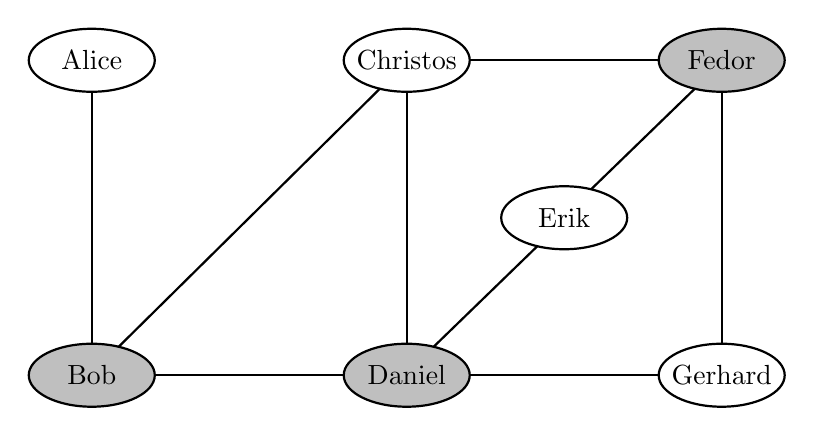
\begin{tikzpicture}[scale=2]
\draw[thick, fill=lightgray] (1,1) ellipse (0.4 and 0.2) node {Bob};
\draw[thick, fill=lightgray] (3,1) ellipse (0.4 and 0.2) node {Daniel};
\draw[thick] (5,1) ellipse (0.4 and 0.2) node {Gerhard};
\draw[thick] (4,2) ellipse (0.4 and 0.2) node {Erik};
\draw[thick] (1,3) ellipse (0.4 and 0.2) node {Alice};
\draw[thick] (3,3) ellipse (0.4 and 0.2) node {Christos};
\draw[thick, fill=lightgray] (5,3) ellipse (0.4 and 0.2) node {Fedor};

\draw[thick] (1.4,1) -- (2.6,1);
\draw[thick] (3.4,1) -- (4.6,1);
\draw[thick] (3.4,3) -- (4.6,3);

\draw[thick] (1,1.2) -- (1,2.8);
\draw[thick] (3,1.2) -- (3,2.8);
\draw[thick] (5,1.2) -- (5,2.8);

\draw[thick] (1.17,1.18) -- (2.83,2.82);
\draw[thick] (3.17,1.18) -- (3.83,1.82);
\draw[thick] (4.17,2.18) -- (4.83,2.82);

\end{tikzpicture}
\end{center}

\end{frame}

